\chapter{Design}

\section{Specification}
\begin{enumerate}
    \item The traffic light control system should be easy to use.
    \item The traffic light control system should be as efficient as possible, reducing heat dissipated to the environment.
    \item The traffic light control system should recieve an input from a pedestrian and take 40 seconds ($\pm$20s) to allow them to cross.
    \item The traffic light control system should not favour any particular road user over an other as well as giving equal chances to all direction of traffic.
    \item The traffic light system should ensure that when a direction of traffic is not able to go, its red stop LED is illuminated.
    \item The traffic light control system should take a 0V and +5V (within $\pm$0.5V) input.
    \item The traffic light control system should alert 'pedestrians' in at least two different ways that it is their turn to cross.
    \item The traffic light control system should be developed in a way such that, the code is clear to read and understand, to ensure future developments can be carried out easily.
\end{enumerate}

\section{Junction design}
Now I have my specification, I am able to design the junction which I will design the traffic light control system for. I will be using a junction in my home town (Eastbourne) as inspiration.
\subsection{Real Life Junction}
\begin{figure}[H]
    \centering
    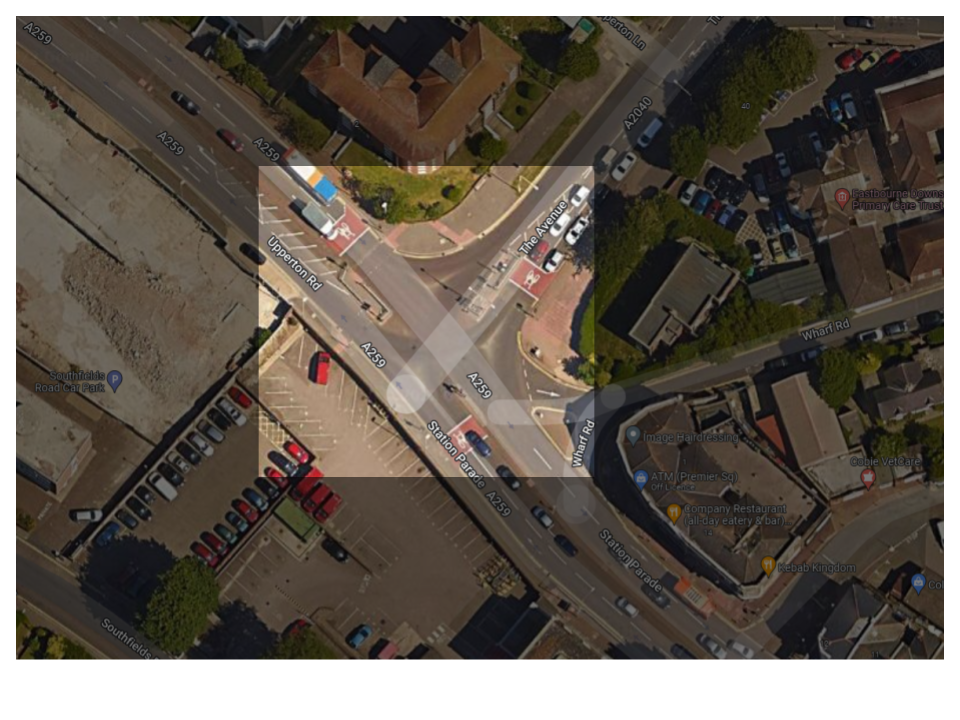
\includegraphics[width=0.9\textwidth]{images/IRL diagram.png}
    \caption{Image of the inspiration junction}
    \label{fig:IRLJunction}
\end{figure}
\noindent \textit{Data from Google Maps (2022). Available from:\\ https://www.google.com/maps/@50.7701274,0.2786944,118m/data=!3m1!1e3 [Accessed 13 03 2022]}\newline

\noindent This is a three-way traffic light controlled junction with pedestrian crossing for two of the three ways. 

\subsection{Abstracted Junction}
\begin{figure}[H]
    \centering
    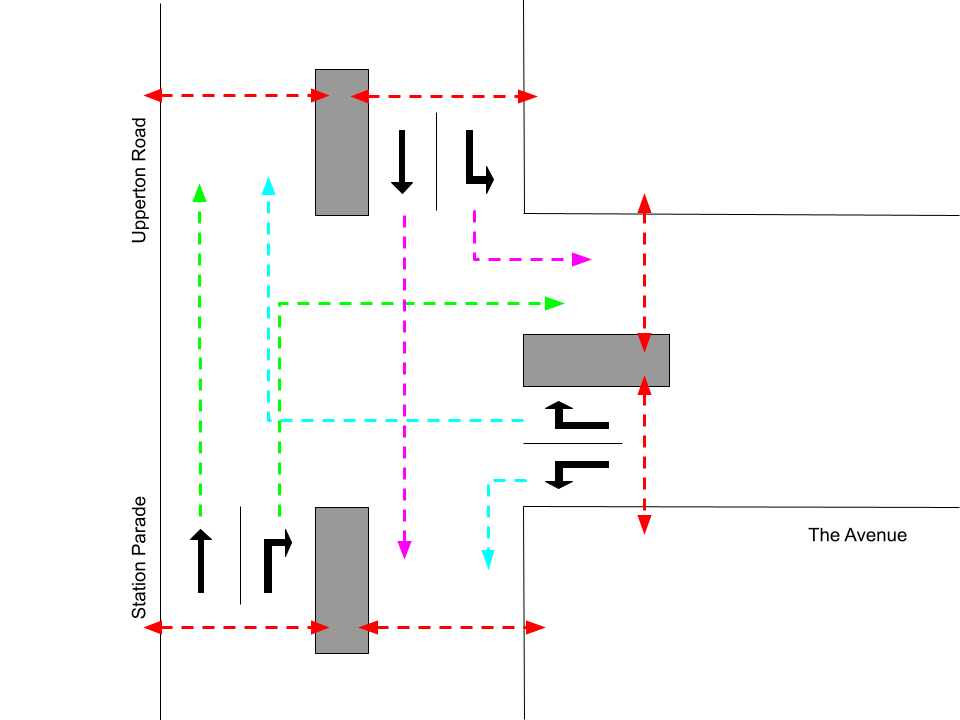
\includegraphics[width=0.8\textwidth]{images/Abstracted diagram.png}
    \caption{Diagram of the junction used in this project}
    \label{fig:abstractedDiagram}
\end{figure}
\noindent The diagram above shows an abstracted version of the junction shows in figure \ref{fig:IRLJunction}. This abstracted version has four colours dashed lines drawn on it. These show the routes which can be taken by either the pedestrians or cars. The red route indicates a pedestrian crossing. The blue, pink and green lines indicate routes which can be taken by vehicles. The grey boxes indicate pedestrian islands. Additional pedestrian crossing routes have been included in my abstracted diagram. This is because in the real junction, the areas which do not have pedestrian crossings are extremely dangerous as cars travel at high speeds.

\section{Traffic Light Sequence}
After working out the type of junction I will design an traffic light control system for, I am now able to work out the sequence which the traffic lights will cycle through. At this point, I have also decided that the traffic light sequence will be contained within a subroutine; hence the references about 'Main Program' in the diagram below.
\begin{figure}[H]
    \centering
    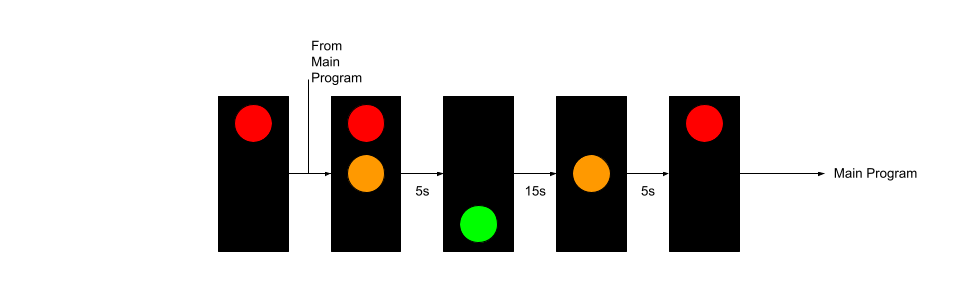
\includegraphics[width=0.9\textwidth]{images/Traffic light sequence.png}
    \caption{Sequence of lights in the traffic lights}
    \label{fig:trafficLightSequence}
\end{figure}

\section{Inputs and Outputs}
The PIC16F88 microcontroller has 16 input output bits, divided into two 'ports' of 8 (PORTA and PORTB).
In my system, all inputs and outputs will be active high (logic 1).
\begin{figure}[H]
    \begin{minipage} {0.45\textwidth}
        \subsection{PORTA}
        \begin{itemize}
            \item[0] Output, red LED
            \item[1] Output, amber LED
            \item[2] Output, green LED
            \item[3] Output, red LED
            \item[4] Output, amber LED
            \item[5] 
            \item[6] Output, red LED
            \item[7] Output, amber LED
        \end{itemize}
    \end{minipage}\hfill
    \begin{minipage} {0.45\textwidth}
        \subsection{PORTB}
        \begin{itemize}
            \item[0] Output, green LED
            \item[1] Input, button
            \item[2] Output, white LED
            \item[3] Output, red LED
            \item[4] Output, green LED
            \item[5] Output, buzzer
            \item[6] 
            \item[7] Output, green LED
        \end{itemize}
    \end{minipage}
\end{figure}


\section{Component of the control system}
The control system will be based off of a PIC16F88 microcontroller, this will be the heart of the system. Alongside the microcontroller, I will also need some LEDs (in red, amber and green), a buzzer and a button.
\subsection{Components list}
\begin{itemize}
    \item 4 red LEDs
    \item 4 green LEDs
    \item 3 amber LEDs
    \item 1 white LED
    \item 2 eight 220K$\Omega$ resistor packs
    \item 3 220k$\Omega$ resistors
    \item 1 1K$\Omega$ resistor
    \item 1 Push-To-Make button
    \item 1 PIC16F88 Microcontroller
\end{itemize}
In reality, my circuit will only need 12 220K$\Omega$ resistors. However, for convenience, and minimising the number of components on the breadboards, it is easier to use 2 resistor packs and a number of loose resistors.


